\let\lesson\undefined
\newcommand{\lesson}{\phantomlesson{Bài 1.}}


\setcounter{section}{2}
\section{Bài tập trắc nghiệm}
\begin{enumerate}[label=\bfseries Câu \arabic*:,leftmargin=1.7cm]
\item \mkstar{1}\\
Chuyển động của các nguyên tử, phân tử trong mô hình động học phân tử được gọi là chuyển động
\begin{mcq}(2)
	\item chuyển động cơ.
	\item chuyển động nhiệt.
	\item chuyển động tròn.
	\item chuyển động đều.
\end{mcq}
\hideall{
\textbf{Đáp án B.}
}

\item \mkstar{1}\\
Chọn phát biểu \textbf{đúng} về lực tương tác giữa các phân tử.
\begin{mcq}
	\item Giữa các phân tử có cả lực hút và lực đẩy.
	\item Giữa các phân tử chỉ có lực hút hoặc lực đẩy.
	\item Giữa các phân tử chỉ có lực đẩy.
	\item Giữa các phân tử chỉ có lực hút.
\end{mcq}
\hideall{
\textbf{Đáp án A.}
}

\item \mkstar{1}\\
Khi khoảng cách giữa các phân tử rất nhỏ, thì giữa các phân tử
\begin{mcq}
	\item chỉ có lực hút.
	\item chỉ có lực đẩy.
	\item có cả lực hút và lực đẩy, nhưng lực đẩy lớn hơn lực hút.
	\item có cả lực hút và lực đẩy, nhưng lực đẩy nhỏ hơn lực hút.
\end{mcq}
\hideall{
\textbf{Đáp án C.}
}

\item \mkstar{1}\\
Mục đích của thí nghiệm Brown là
\begin{mcq}
	\item quan sát hạt phấn hoa bằng kính hiển vi.
	\item quan sát chuyển động của hạt phấn hoa trong nước bằng kính hiển vi.
	\item quan sát cánh hoa trong nước bằng kính hiển vi.
	\item quan sát chuyển động của cánh hoa.
\end{mcq}
\hideall{
\textbf{Đáp án B.}
}

\item  \mkstar{1}\\
Trong thí nghiệm của Brown các hạt phấn hoa chuyển động hỗn độn, không ngừng vì
\begin{mcq}
	\item giữa các hạt phấn hoa có lực tương tác hút và đẩy.
	\item các hạt phấn hoa là các thực thể sống.
	\item các phân tử nước chuyển động không ngừng, va chạm vào chúng từ mọi phía.
	\item các hạt phấn hoa có thể dao động tự do quanh vị trí cân bằng.
\end{mcq}
\hideall{
\textbf{Đáp án C.}
}

\item\mkstar{1}\\
Chọn câu trả lời \textbf{đúng nhất}. \\
Các chất có thể tồn tại ở những thể nào?
\begin{mcq}
	\item Thể rắn, thể lỏng, thể khí hoặc chân không.
	\item Thể rắn, thể lỏng hoặc thể khí.
	\item Thể rắn và thể hơi.
	\item Thể rắn và thế lỏng.
\end{mcq}
\hideall{
\textbf{Đáp án B.}
}



\item \mkstar{1}
Đặc điểm nào sau đây là phù hợp với chất rắn?
\begin{mcq}
	\item Có lực tương tác giữa các phân tử rất mạnh.
	\item Có lực tương tác giữa các phân tử rất yếu.
	\item Không có hình dạng xác định.
	\item Không có thể tích riêng xác định.
\end{mcq}
\hideall{
\textbf{Đáp án A.}
}

\item \mkstar{1}\\
Phát biểu nào dưới đây là đúng khi nói về những đặc điểm của chất rắn?
\begin{mcq}
	\item Có khối lượng, hình dạng xác định, không có thể tích xác định.
	\item Có khối lượng xác định, hình dạng và thể tích không xác định.
	\item Có khối lượng, hình dạng, thể tích xác định.
	\item Có khối lượng và thể tích xác định, hình dạng không xác định.
\end{mcq}
\hideall{
\textbf{Đáp án C.}
}



\item \mkstar{1}\\
Người ta có thể phân loại chất rắn một cách tổng quát theo cách nào sau đây?
\begin{mcq}
	\item Chất rắn đơn tinh thể và chất rắn vô định hình.
	\item Chất rắn kết tinh và chất rắn vô định hình.
	\item Chất rắn đa tinh thể và chất rắn vô định hình.
	\item Chất rắn đơn tinh thể và chất rắn đa tinh thể.
\end{mcq}
\hideall{
\textbf{Đáp án B.}
}



\item \mkstar{1}\\
Đặc điểm nào sau đây là đặc điểm cấu trúc phân tử ở thể lỏng?
\begin{mcq}
	\item Khoảng cách giữa các phân tử rất lớn so với kích thước của chúng.
	\item Lực tương tác phân tử yếu hơn lực tương tác phân tử ở thể rắn.
	\item Không có thể tích và hình dạng riêng xác định.
	\item Các phân tử dao động xung quanh vị trí cân bằng xác định.
\end{mcq}
\hideall{
\textbf{Đáp án B.}
}

\item \mkstar{1}\\
Trong chuyển động nhiệt, các phân tử chất lỏng
\begin{mcq}
	\item dao động quanh vị trí cân bằng xác định.
	\item chuyển động hỗn loạn quanh vị trí cân bằng xác định.
	\item chuyển động hỗn loạn.
	\item dao động quanh vị trí cân bằng nhưng những vị trí này không cố định mà luôn thay đổi.
\end{mcq}
\hideall{
\textbf{Đáp án D.}
}

\item \mkstar{1}\\
Chất lỏng có thể tích xác định, nhưng hình dạng không xác định là do trong chất lỏng
\begin{mcq}
	\item lực liên kết giữa các phân tử chất lỏng là rất lớn, các phân tử chỉ dao động không ngừng quanh một vị trí xác định.
	\item lực liên kết giữa các phân tử chất lỏng là rất yếu, các phân tử dao động tự do về mọi phía.
	\item lực liên kết giữa các phân tử chất lỏng là yếu hơn chất rắn, các phân tử dao động tương đối
	tự do hơn so với trong chất rắn.
	\item Tất cả các phương án đưa ra đều sai.
\end{mcq}
\hideall{
\textbf{Đáp án C.}
}

\item \mkstar{1}\\
Các phân tử khí chuyển động hỗn loạn, không ngừng vì
\begin{mcq}
	\item phân tử khí không có khối lượng.
	\item khoảng cách giữa các phân tử khí quá gần nhau.
	\item lực tương tác giữa các phân tử quá nhỏ.
	\item các phân tử khí luôn đẩy nhau.
\end{mcq}
\hideall{
\textbf{Đáp án C.}
}

\item \mkstar{1}\\
Tính chất nào sau đây \textbf{không phải} là tính chất của chất ở thể khí?
\begin{mcq}
	\item Có hình dạng và thể tích riêng.
	\item Có các phân tử chuyển động hoàn toàn hỗn độn.
	\item Có thể nén được dễ dàng.
	\item Có lực tương tác phân tử nhỏ hơn lực tương tác phân tử ở thể rắn và thể lỏng.
\end{mcq}
\hideall{
\textbf{Đáp án A.}
}

\item \mkstar{1}\\
Chất khí không có hình dạng và thể tích riêng là vì
\begin{mcq}
	\item khoảng cách giữa các phân tử rất gần, lực tương tác giữa các phân tử chất khí rất mạnh.
	\item khoảng cách giữa các phân tử rất gần, lực tương tác giữa các phân tử chất khí rất yếu.
	\item khoảng cách giữa các phân tử rất xa, lực tương tác giữa các phân tử chất khí rất mạnh.
	\item khoảng cách giữa các phân tử rất xa, lực tương tác giữa các phân tử chất khí rất yếu.
\end{mcq}
\hideall{
\textbf{Đáp án D.}
}

\item \mkstar{1}\\
Khi mở nắp lọ nước hoa, ta có thể ngửi thấy mùi thơm tràn ngập trong phòng. Điều này thể hiện tính chất nào của chất khí?
\begin{mcq}
	\item Dễ dàng nén được.
	\item Có khối lượng xác định.
	\item Có thể khuếch tán trong không gian theo mọi hướng.
	\item Không chảy được.
\end{mcq}
\hideall{
\textbf{Đáp án C.}
}

\item \mkstar{1}\\
Sự nóng chảy là
\begin{mcq}(2)
	\item sự chuyển thế từ rắn sang lỏng.
	\item sự chuyển thể từ rắn sang khí.
	\item sự chuyển thể từ lỏng sang rắn.
	\item sự chuyển thể từ lỏng sang khí.
\end{mcq}
\hideall{
\textbf{Đáp án A.}
}

\item \mkstar{1}\\
Sự đông đặc là
\begin{mcq}(2)
	\item sự chuyển thế từ rắn sang lỏng.
	\item sự chuyển thể từ rắn sang khí.
	\item sự chuyển thể từ lỏng sang rắn.
	\item sự chuyển thể từ lỏng sang khí.
\end{mcq}
\hideall{
	\textbf{Đáp án C.}
}

\item \mkstar{1}\\
Sự bay hơi là
\begin{mcq}(2)
	\item sự chuyển thế từ rắn sang lỏng.
	\item sự chuyển thể từ rắn sang khí.
	\item sự chuyển thể từ lỏng sang rắn.
	\item sự chuyển thể từ lỏng sang khí.
\end{mcq}
\hideall{
	\textbf{Đáp án D.}
}



\item \mkstar{1}\\
Khi quan sát sự nóng chảy của nước đá, trong suốt thời gian nóng chảy thì
\begin{mcq}
	\item nhiệt độ của nước đá tăng.
	\item nhiệt độ của nước đá giảm.
	\item nhiệt  độ của nước đá không đổi.
	\item nhiệt độ của nước đá ban đầu tăng và sau đó giảm.
\end{mcq}
\hideall{
\textbf{Đáp án C.}
}

\item\mkstar{1}\\
 Phát biểu nào sau đây về tính chất của chất rắn kết tinh và chất rắn vô định hình là \textbf{đúng}?
\begin{mcq}
	\item Chất rắn kết tinh và chất rắn vô định hình đều có nhiệt độ nóng chảy xác định.
	\item Chất rắn kết tinh không có nhiệt độ nóng chảy xác định, chất rắn vô định hình có nhiệt độ nóng chảy
	xác định.
	\item Chất rắn kết tinh có nhiệt độ nóng chảy xác định, chất rắn vô định hình không có nhiệt độ nóng chảy
	xác định.
	\item Chất rắn kết tinh và chất rắn vô định hình đều không có nhiệt độ nóng chảy xác định.
\end{mcq}
\hideall{
\textbf{Đáp án C.}
}

\item \mkstar{1}\\
Một vật rắn khi bị nung nóng thì mềm dần. Đó là
\begin{mcq}(2)
	\item chất rắn kết tinh.
	\item chất rắn đơn tinh thể.
	\item chất rắn đa tinh thể.
	\item chất rắn vô định hình.
\end{mcq}
\hideall{
\textbf{Đáp án D.}
}

	

\item \mkstar{1}\\
Trường hợp nào sau đây không liên quan đến sự nóng chảy và đông đặc?
\begin{center}
	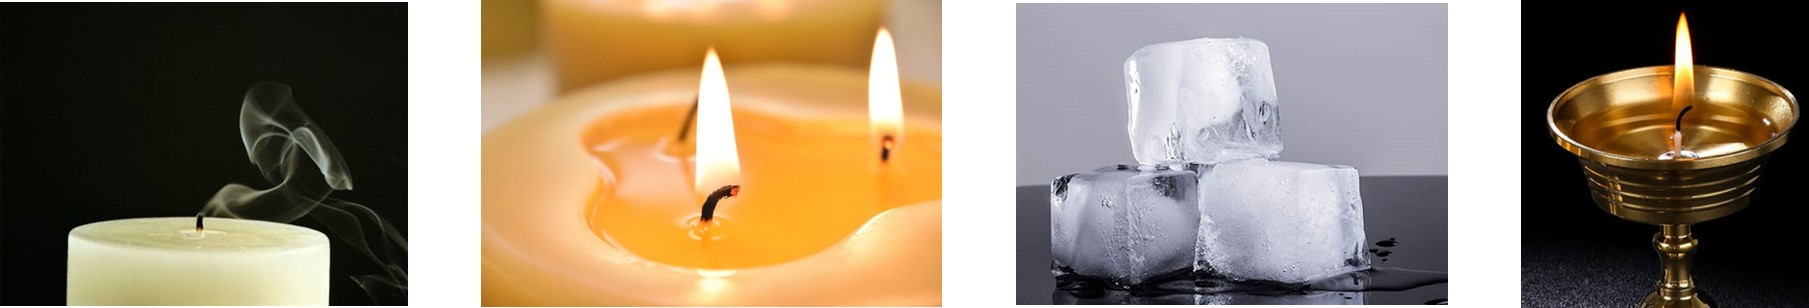
\includegraphics[width=0.45\linewidth]{../figs/VN12-Y24-PH-SYL-001P-2}
\end{center}
\begin{mcq}(2)
	\item Ngọn nến vừa tắt.
	\item Ngọn nến đang cháy.
	\item Nước đá vừa lấy ra khỏi tủ lạnh.
	\item Ngọn đèn dầu đang cháy.
\end{mcq}
\hideall{
\textbf{Đáp án D.}
}


\item \mkstar{1}\\
Sự bay hơi diễn ra càng nhanh hơn khi
\begin{mcq}(2)
	\item nhiệt độ càng thấp.
	\item tốc độ gió càng lớn.
	\item lượng chất lỏng càng nhiều.
	\item diện tích mặt thoáng càng hẹp.
\end{mcq}
\hideall{
\textbf{Đáp án B.}
}

\item \mkstar{1}\\
Một ấm nước đang sôi, nếu tiếp tục đun thì
\begin{mcq}(2)
	\item nhiệt độ nước trong ấm giảm xuống.
	\item nước trong ấm không bay hơi nữa.
	\item nhiệt độ nước trong ấm vẫn tiếp tục tăng.
	\item nước trong ấm bay hơi nhiều hơn và cạn dần.
\end{mcq}
\hideall{
\textbf{Đáp án D.}
}



\item \mkstar{1}\\
Phát biểu nào sau đây là \textbf{không đúng} về sự bay hơi?
\begin{mcq}
	\item Sự bay hơi là quá trình chuyển từ thể lỏng sang thể khí xảy ra ở bề mặt chất lỏng.
	\item Sự bay hơi là quá trình chuyển từ thể lỏng sang thể khí xảy ra ở cả bên trong và trên bề mặt
	chất lỏng.
	\item Sự bay hơi của chất lỏng xảy ra ở nhiệt độ bất kì.
	\item Sự ngưng tụ luôn kèm theo sự bay hơi.
\end{mcq}
\hideall{
\textbf{Đáp án B.}
}

\item \mkstar{1}\\
Sự sôi xảy ra ở
\begin{mcq}(4)
	\item nhiệt độ trên $\SI{100}{\celsius}$.
	\item $\SI{100}{\celsius}$.
	\item nhiệt độ sôi.
	\item dưới $\SI{100}{\celsius}$.
\end{mcq}
\hideall{
\textbf{Đáp án C.}
}

\item \mkstar{1}\\
Trong các trường hợp dưới đây, trường hợp nào liên quan đến sự bay hơi?
\begin{mcq}
	\item Kính cửa sổ bị mờ đi trong những ngày đông giá lạnh.
	\item Dầu trong đèn bị khô cạn dù không sử dụng.
	\item Miếng bơ để bên ngoài tủ lạnh sau một thời gian bị chảy lỏng.
	\item Đưa nước vào trong tủ lạnh để làm đá.
\end{mcq}
\hideall{
\textbf{Đáp án B.}
}

\item \mkstar{2}\\
Tại sao quả bóng bay dù buộc chặt để lâu ngày vẫn bị xẹp?
\begin{mcq}
	\item Vì khi mới thổi, không khí từ miệng vào bóng còn nóng, sau đó lạnh dần nên co lại.
	\item Vì cao su là chất đàn hồi nên sau khi bị thổi căng nó tự động co lại.
	\item Vì không khí nhẹ nên có thể chui qua chỗ buộc ra ngoài.
	\item Vì giữa các phân tử của chất làm vỏ bóng có khoảng cách nên các phân tử không khí có thể chui qua đó và thoát ra ngoài.
\end{mcq}
\hideall{
	\textbf{Đáp án D.}
}

\item \mkstar{2}\\
Hãy chọn phương án \textbf{sai}.\\
Cùng một khối lượng của một chất nhưng khi ở các thể khác nhau thì sẽ khác nhau
\begin{mcq}(2)
	\item Thể tích.
	\item Khối lượng riêng.
	\item Kích thước của các nguyên tử.
	\item Trật tự của các nguyên tử.
\end{mcq}
\hideall{
	\textbf{Đáp án C.}
}

\item \mkstar{2}\\
Các nguyên tử trong một miếng sắt có tính chất nào sau đây?
\begin{mcq}(2)
	\item Khi nhiệt độ tăng thì nở ra.
	\item Khi nhiệt độ giảm thì co lại.
	\item Đứng rất gần nhau.
	\item Đứng xa nhau.
\end{mcq}
\hideall{
	\textbf{Đáp án C.}
}

\item \mkstar{2}\\
Trong các chất sau, chất nào \textbf{không phải} là chất rắn kết tinh?
\begin{mcq}(4)
	\item Muối ăn.
	\item Thuỷ tinh.
	\item Kim cương.
	\item Thạch anh.
\end{mcq}
\hideall{
	\textbf{Đáp án B.}
}

\item \mkstar{2}\\
Chất rắn nào dưới đây không phải là chất rắn vô định hình?
\begin{mcq}(4)
	\item Thạch anh.
	\item Thuỷ tinh.
	\item Sáp.
	\item Cao su.
\end{mcq}
\hideall{
	\textbf{Đáp án A.}
}

\item \mkstar{2}\\
Chất rắn nào dưới đây là chất rắn vô định hình?
\begin{mcq}(4)
	\item Muối ăn.
	\item Kim loại.
	\item Thạch anh.
	\item Nhựa đường.
\end{mcq}
\hideall{
	\textbf{Đáp án D.}
}

\item \mkstar{2}\\
Ở điều kiện thường, iode là chất rắn dạng tinh thể màu đen tím. Khi đun nóng, iode có sự thăng hoa.\\
Vậy sự thăng hoa của iode là sự chuyển trạng thái từ thể
\begin{mcq}(4)
	\item rắn sang khí.
	\item rắn sang lỏng.
	\item lỏng sang rắn.
	\item khí sang rắn.
\end{mcq}
\hideall{
	\textbf{Đáp án A.}
}

\item \mkstar{2}\\
Cho đồ thị biểu diễn sự thay đổi nhiệt độ theo thời gian của nước đá như hình vẽ. Nước đá tan trong khoảng thời gian nào?
\begin{center}
	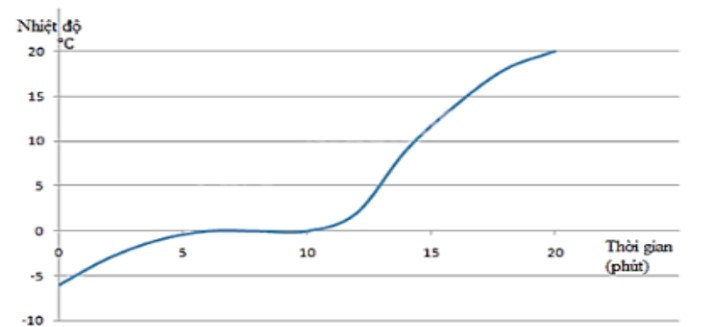
\includegraphics[width=0.6\linewidth]{../figs/VN12-Y24-PH-SYL-001P-1}
\end{center}
\begin{mcq}(2)
	\item Từ phút thứ 6 đến phút thứ 10.
	\item Từ phút thứ 10 trở đi.
	\item Từ 0 đến phút thứ 6.
	\item Từ phút thứ 10 đến phút thứ 15.
\end{mcq}
\hideall{
	\textbf{Đáp án A.}
}

\item \mkstar{2}\\
Người ta không thể luộc trứng chín ở núi cao vì
\begin{mcq}
	\item áp suất trên núi thấp hơn áp suất chuẩn $\left(\SI{1}{atm}\right)$ nên nước sôi ở nhiệt độ thấp hơn $\SI{100}{\celsius}$.
	\item áp suất trên núi cao hơn áp suất chuẩn $\left(\SI{1}{atm}\right)$ nên nước sôi ở nhiệt độ thấp hơn $\SI{100}{\celsius}$.
	\item áp suất trên núi thấp hơn áp suất chuẩn $\left(\SI{1}{atm}\right)$ nên nước sôi ở nhiệt độ cao hơn $\SI{100}{\celsius}$.
	\item áp suất trên núi cao hơn áp suất chuẩn $\left(\SI{1}{atm}\right)$ nên nước sôi ở nhiệt độ cao hơn $\SI{100}{\celsius}$.
\end{mcq}
\hideall{
	\textbf{Đáp án A.}
}

\item \mkstar{2}\\
Thuỷ ngân có nhiệt độ nóng chảy là $\SI{-39}{\celsius}$ và nhiệt độ sôi là $\SI{357}{\celsius}$. Khi ở trong phòng có nhiệt độ $\SI{30}{\celsius}$ thì thuỷ ngân
\begin{mcq}(2)
	\item chỉ tồn tại ở thể lỏng.
	\item chỉ tồn tại ở thể hơi.
	\item tồn tại ở cả thể lỏng và thể hơi.
	\item tồn tại ở cả thể rắn, lỏng và hơi.
\end{mcq}
\hideall{
	\textbf{Đáp án A.}
}

\item \mkstar{2}\\
Tại sao khi cầm vào vỏ bình ga mini đang sử dụng ta thường thấy có một lớp nước rất
mỏng trên đó?
\begin{mcq}
	\item Do hơi nước từ tay ta bốc ra.
	\item Nước từ trong bình ga thấm ra.
	\item Do vỏ bình ga lạnh hơn nhiệt độ môi trường nên hơi nước trong không khí ngưng tụ trên đó.
	\item Cả B và C đều đúng.
\end{mcq}
\hideall{
	\textbf{Đáp án C.}
}

\item \mkstar{2}\\
Ở nhiệt độ trong phòng, chỉ có thể có khí oxygen, không thể có oxygen lỏng vì
\begin{mcq}(2)
	\item oxygen luôn là chất khí.
	\item nhiệt độ phòng cao hơn nhiệt độ sôi của oxygen.
	\item nhiệt độ phòng thấp hơn nhiệt độ sôi của oxygen.
	\item nhiệt độ trong phòng bằng nhiệt độ sôi của oxygen.
\end{mcq}
\hideall{
\textbf{Đáp án B.}
}
\end{enumerate}
\section{Trắc nghiệm đúng/sai}
\begin{enumerate}[label=\bfseries Câu \arabic*:, leftmargin=1.7cm]
	\item\mkstar{1}\\
	Nhận định các phát biểu sau đây về mô hình động học phân tử.
	\begin{enumerate}[label=\alph*)]
		\item Các chất được cấu tạo từ các hạt riêng biệt được gọi nguyên tử, phân tử.
		\item Các nguyên tử, phân tử đứng sát nhau và giữa chúng không có khoảng cách.
		\item Lực tương tác giữa các phân tử ở thể rắn lớn hơn lực tương tác giữa các phân tử ở thể lỏng và thể khí.
		\item Các nguyên tử, phân tử chất lỏng dao động xung quanh các vị trí cân bằng không cố định.
	\end{enumerate}
\hideall{
\begin{enumerate}[label=\alph*)]
	\item Đúng.
	\item Sai.
	\item Đúng.
	\item Đúng.
\end{enumerate}
}

\item \mkstar{1}\\
Nhận định các phát biểu về sự sôi.
\begin{enumerate}[label=\alph*)]
	\item Nước chỉ sôi ở nhiệt độ $\SI{100}{\celsius}$.
	\item Trong suốt thời gian sôi, nhiệt độ của nước không thay đổi.
	\item Nước chỉ bay hơi ở nhiệt độ sôi.
	\item Trong suốt thời gian sôi, nước vừa bay hơi tạo ra bọt khí và vừa bay hơi trên bề mặt.
\end{enumerate}
\hideall{
\begin{enumerate}[label=\alph*)]
	\item Sai. Nhiệt độ sôi của nước còn phụ thuộc vào áp suất nơi đun.
	\item Đúng.
	\item Sai. Nước bay hơi ở bất kì nhiệt độ nào.
	\item Đúng.
\end{enumerate}
}

\item \mkstar{2}\\
Hình bên là đồ thị biểu diễn sự thay đổi nhiệt độ của nước theo thời gian đun.
\begin{center}
	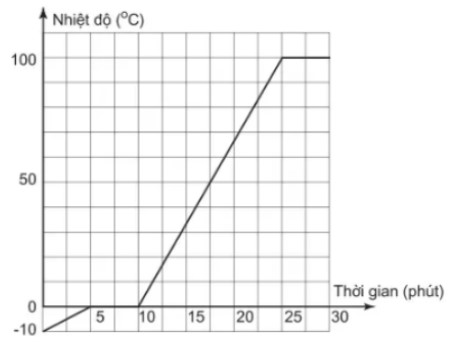
\includegraphics[width=0.45\linewidth]{../figs/VN12-Y24-PH-SYL-001P-4}
\end{center}
\begin{enumerate}[label=\alph*)]
	\item Trong 5 phút đầu tiên, nước ở thể rắn.
	\item Từ phút thứ 5 đến phút thứ 10 nước đá nóng chảy.
	\item Từ phút thứ 10 đến phút thứ 25 nước không có sự bay hơi vì chưa đạt nhiệt độ sôi.
	\item Nước được đun ở điều kiện tiêu chuẩn.
\end{enumerate}
\hideall{
	\begin{enumerate}[label=\alph*)]
		\item Đúng.
		\item Đúng.
		\item Sai. Nước bay hơi ở bất kì nhiệt độ nào.
		\item Đúng. Đồ thị thể hiện quá trình nước sôi ở $\SI{100}{\celsius}$.
	\end{enumerate}
}

\item \mkstar{2}\\
Bảng dưới đây ghi nhận nhiệt độ nóng chảy và nhiệt độ sôi của một số chất
\begin{center}
	\begin{tabular}{|C{8em}|C{10em}|C{8em}|}
		\hline
		\thead{Chất}& \thead{Nhiệt độ nóng chảy} &\thead{Nhiệt độ sôi}\\
		\hline
		Chì & $\SI{327}{\celsius}$ & $\SI{1613}{\celsius}$\\
		\hline
		Nước & $\SI{0}{\celsius}$ & $\SI{100}{\celsius}$\\
		\hline
		Oxide & $\SI{-219}{\celsius}$ & $\SI{-183}{\celsius}$\\
		\hline
		Rượu & $\SI{-117}{\celsius}$ & $\SI{78}{\celsius}$\\
		\hline
		Thuỷ ngân & $\SI{-39}{\celsius}$ & $\SI{357}{\celsius}$\\
		\hline
	\end{tabular}
\end{center}
\begin{enumerate}[label=\alph*)]
	\item Chì có nhiệt độ sôi cao nhất trong các chất được liệt kê.
	\item Nước có nhiệt độ sôi thấp nhất trong các chất được liệt kê.
	\item Ở nhiệt độ $\SI{30}{\celsius}$ thì chì ở thể  rắn.
	\item Ở nhiệt độ $\SI{30}{\celsius}$ thì oxide ở thể lỏng.
\end{enumerate}
\hideall{
	\begin{enumerate}[label=\alph*)]
		\item Đúng.
		\item Sai.
		\item Đúng.
		\item Sai. 
	\end{enumerate}
}
	
	\item \mkstar{2}\\
	Hình bên là một cốc nước đá đặt ngoài không khí.
	\begin{center}
		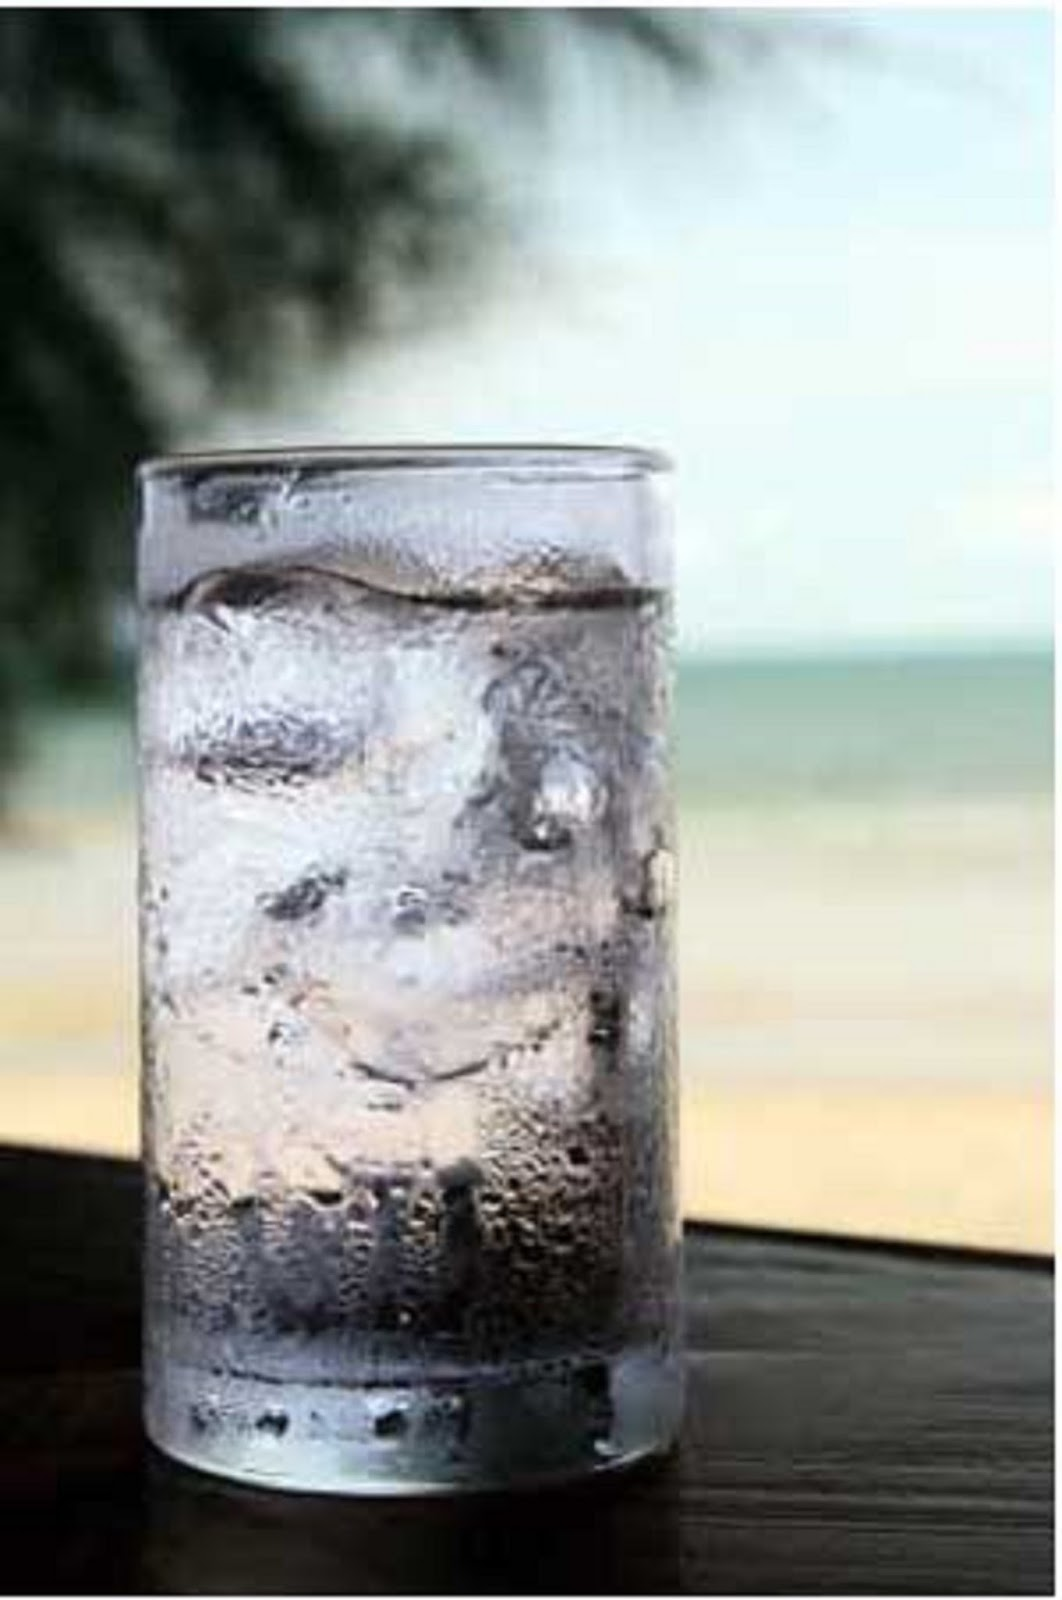
\includegraphics[width=0.2\linewidth]{../figs/VN12-Y24-PH-SYL-001P-3}
	\end{center}
\begin{enumerate}[label=\alph*)]
	\item 
	Nước ngưng đọng trên thành cốc là do nước bên trong cốc thấm ra ngoài.
	\item Nước đá truyền nhiệt ra bên ngoài làm đá tan dần.
	\item Khói trắng xuất hiện trên miệng cốc là do sự hoá hơi của nước trong cốc.
	\item Khi đá chưa tan hết thì nhiệt độ của nước trong cốc là $\SI{0}{\celsius}$.
\end{enumerate}
\hideall{
\begin{enumerate}[label=\alph*)]
	\item Sai. Nước đọng trên thành cốc là do hơi nước trong không khí gần cốc ngưng tụ.
	\item Sai. Nước đá nhận nhiệt từ môi trường nên tan dần.
	\item Sai. Khói trắng xuất hiện ở miệng cốc là kết quả sự ngưng tụ của hơi nước trong không khí.
	\item Đúng.
\end{enumerate}
}




\end{enumerate}
\section{Bài tập tự luận}
\begin{enumerate}[label=\bfseries Câu \arabic*:,leftmargin=1.7cm]
	\item Hãy sử dụng mô hình động học phân tử để giải thích vì sao chúng ta có thể đi trong không khí, bơi trong nước nhưng không thể đi xuyên qua tường?
	\hideall{
		Lực liên kết giữa các phân tử chất rắn lớn hơn nhiều so với lực liên kết giữa các phân tử chất lỏng và chất khí. Do đó, ta khó bẽ gãy được liên kết của các phân tử chất rắn nên không thể đi xuyên qua tường.
		
	}
	
	\item Cùng một chất, khi ở thể lỏng thường có khối lượng riêng nhỏ hơn khi ở thể rắn và khối lượng riêng ở thế khí lại nhỏ hơn khi ở thể lỏng. Vì sao như vậy?
	\hideall{Vì khoảng cách trung bình giữa các phân tử chất khí lớn hơn khoảng cách trung bình giữa các phân tử chất lỏng và lớn hơn khoảng cách trung bình giữa các phân tử chất rắn. Do đó, với cùng một chất thì thể khí thường có thể tích lớn hơn so với với thể lỏng và lớn hớn thể tích ở rắn. Vì vậy, ở thể lỏng thường có khối lượng riêng nhỏ hơn khi ở thể rắn và khối lượng riêng ở thế khí lại nhỏ hơn khi ở thể lỏng.
		\luuy{Không đúng cho tất cả trường hợp. Ví dụ, nước có thể tích ở thể rắn lớn hơn thể tích ở thể lỏng.}
		
	}
	
	\item Cồn y tế chuyển từ thể lỏng sang thể khí rất nhanh ở điều kiện thông thường. Hãy giải thích tại sao khi xoa cồn vào da, ta cảm thấy lạnh ở vùng da đó?
	\hideall{
		Khi cồn chuyển thể từ lỏng sang khí thì cần thu nhiệt lượng, do đó tay ta mất bớt nhiệt lượng truyền cho cồn và cảm thấy vùng da thoa cồn bị lạnh đi.
		
	}
	
	\item Vì sao bình nước sôi muốn để nguội nhanh thì cần mở nắp để hơi nước thoát ra?
	\hideall{
		Vì hơi nước có nhiệt độ cao, khi mở nắp thì hơi nước thoát ra nhiều và nhanh hơn làm cho nước còn lại trong bình dễ trao đổi nhiệt với không khí bên ngoài và giảm nhanh nhiệt độ.
	}
	
	
	\item Rau xanh sau khi mua về thường bị héo khi để ở ngoài trời nắng. Vì sao lại có hiện tượng trên? Làm thế nào để hạn chế điều này?
	\hideall{
		Rau bị héo là do sự bay hơi của nước trong rau qua bề mặt lá. Để hạn chế rau nhanh héo có thể thực hiện các cách sau
		\begin{itemize}
			\item Tránh ánh nắng trực tiếp từ mặt trời, bảo quản ở nơi thoáng mát.
			\item Vẫy nước lên rau để tạo lớp nước bám trên bề mặt, lớp nước này sẽ hấp thụ nhiệt từ môi trường và bay hơi trước.
		\end{itemize}
		
	}
	
	\item Để khử trùng các dụng cụ y tế nhiều lần (kéo, kẹp gắp, dao mổ, \dots), ngày nay người ta thường sấy chúng trong lò sấy ở nhiệt độ cao. Tuy nhiên, trước đây người ta thường phải luộc chúng trong nước sôi. Giả sử cần phải thực hiện nhiệm vụ này nhưng có một số vi khuẩn chỉ bị tiêu diệt ở nhiệt độ $\SI{105}{\celsius}$, trong đó khi nhiệt độ sôi của nước ở điều kiện tiêu chuẩn là $\SI{100}{\celsius}$. Hãy đề xuất phương án đơn giản để diệt các vi khuẩn này và giải thích.
\hideall{
Tăng áp suất đun nước (dùng nối áp suất) để tăng nhiệt độ sôi của nước.
}
	
	
	\item Một người thợ mộc sau khi đánh vecni vào một số chân giường, sau một thời gian, người thợ mộc phát hiện thấy những chân giường chưa được đánh vecni bị nứt (rạn chân chim), còn những chân giường đã được đánh vecni thì không bị như thế. Hãy giải thích tại sao?
	\hideall{
	Trong gỗ có chứa một lượng nước nhất định, khi đánh vecni lên gỗ, lớp vecni ngăn cách sự tiếp xúc của gỗ với môi trường bên ngoài và làm hạn chế sự bay hơi của nước trong gỗ. Còn những chân giường không đánh vecni thì nước trong gỗ bị bay hơi và làm gỗ bị khô, nứt.
}
\end{enumerate}

















